%% template.tex
%% from
%% bare_conf.tex
%% V1.4b
%% 2015/08/26
%% by Michael Shell
%% See:
%% http://www.michaelshell.org/
%% for current contact information.
%%
%% This is a skeleton file demonstrating the use of IEEEtran.cls
%% (requires IEEEtran.cls version 1.8b or later) with an IEEE
%% conference paper.
%%
%% Support sites:
%% http://www.michaelshell.org/tex/ieeetran/
%% http://www.ctan.org/pkg/ieeetran
%% and
%% http://www.ieee.org/

%%*************************************************************************
%% Legal Notice:
%% This code is offered as-is without any warranty either expressed or
%% implied; without even the implied warranty of MERCHANTABILITY or
%% FITNESS FOR A PARTICULAR PURPOSE!
%% User assumes all risk.
%% In no event shall the IEEE or any contributor to this code be liable for
%% any damages or losses, including, but not limited to, incidental,
%% consequential, or any other damages, resulting from the use or misuse
%% of any information contained here.
%%
%% All comments are the opinions of their respective authors and are not
%% necessarily endorsed by the IEEE.
%%
%% This work is distributed under the LaTeX Project Public License (LPPL)
%% ( http://www.latex-project.org/ ) version 1.3, and may be freely used,
%% distributed and modified. A copy of the LPPL, version 1.3, is included
%% in the base LaTeX documentation of all distributions of LaTeX released
%% 2003/12/01 or later.
%% Retain all contribution notices and credits.
%% ** Modified files should be clearly indicated as such, including  **
%% ** renaming them and changing author support contact information. **
%%*************************************************************************


% *** Authors should verify (and, if needed, correct) their LaTeX system  ***
% *** with the testflow diagnostic prior to trusting their LaTeX platform ***
% *** with production work. The IEEE's font choices and paper sizes can   ***
% *** trigger bugs that do not appear when using other class files.       ***                          ***
% The testflow support page is at:
% http://www.michaelshell.org/tex/testflow/

\documentclass[conference,final,]{IEEEtran}
% Some Computer Society conferences also require the compsoc mode option,
% but others use the standard conference format.
%
% If IEEEtran.cls has not been installed into the LaTeX system files,
% manually specify the path to it like:
% \documentclass[conference]{../sty/IEEEtran}





% Some very useful LaTeX packages include:
% (uncomment the ones you want to load)


% *** MISC UTILITY PACKAGES ***
%
%\usepackage{ifpdf}
% Heiko Oberdiek's ifpdf.sty is very useful if you need conditional
% compilation based on whether the output is pdf or dvi.
% usage:
% \ifpdf
%   % pdf code
% \else
%   % dvi code
% \fi
% The latest version of ifpdf.sty can be obtained from:
% http://www.ctan.org/pkg/ifpdf
% Also, note that IEEEtran.cls V1.7 and later provides a builtin
% \ifCLASSINFOpdf conditional that works the same way.
% When switching from latex to pdflatex and vice-versa, the compiler may
% have to be run twice to clear warning/error messages.






% *** CITATION PACKAGES ***
%
%\usepackage{cite}
% cite.sty was written by Donald Arseneau
% V1.6 and later of IEEEtran pre-defines the format of the cite.sty package
% \cite{} output to follow that of the IEEE. Loading the cite package will
% result in citation numbers being automatically sorted and properly
% "compressed/ranged". e.g., [1], [9], [2], [7], [5], [6] without using
% cite.sty will become [1], [2], [5]--[7], [9] using cite.sty. cite.sty's
% \cite will automatically add leading space, if needed. Use cite.sty's
% noadjust option (cite.sty V3.8 and later) if you want to turn this off
% such as if a citation ever needs to be enclosed in parenthesis.
% cite.sty is already installed on most LaTeX systems. Be sure and use
% version 5.0 (2009-03-20) and later if using hyperref.sty.
% The latest version can be obtained at:
% http://www.ctan.org/pkg/cite
% The documentation is contained in the cite.sty file itself.






% *** GRAPHICS RELATED PACKAGES ***
%
\ifCLASSINFOpdf
  % \usepackage[pdftex]{graphicx}
  % declare the path(s) where your graphic files are
  % \graphicspath{{../pdf/}{../jpeg/}}
  % and their extensions so you won't have to specify these with
  % every instance of \includegraphics
  % \DeclareGraphicsExtensions{.pdf,.jpeg,.png}
\else
  % or other class option (dvipsone, dvipdf, if not using dvips). graphicx
  % will default to the driver specified in the system graphics.cfg if no
  % driver is specified.
  % \usepackage[dvips]{graphicx}
  % declare the path(s) where your graphic files are
  % \graphicspath{{../eps/}}
  % and their extensions so you won't have to specify these with
  % every instance of \includegraphics
  % \DeclareGraphicsExtensions{.eps}
\fi
% graphicx was written by David Carlisle and Sebastian Rahtz. It is
% required if you want graphics, photos, etc. graphicx.sty is already
% installed on most LaTeX systems. The latest version and documentation
% can be obtained at:
% http://www.ctan.org/pkg/graphicx
% Another good source of documentation is "Using Imported Graphics in
% LaTeX2e" by Keith Reckdahl which can be found at:
% http://www.ctan.org/pkg/epslatex
%
% latex, and pdflatex in dvi mode, support graphics in encapsulated
% postscript (.eps) format. pdflatex in pdf mode supports graphics
% in .pdf, .jpeg, .png and .mps (metapost) formats. Users should ensure
% that all non-photo figures use a vector format (.eps, .pdf, .mps) and
% not a bitmapped formats (.jpeg, .png). The IEEE frowns on bitmapped formats
% which can result in "jaggedy"/blurry rendering of lines and letters as
% well as large increases in file sizes.
%
% You can find documentation about the pdfTeX application at:
% http://www.tug.org/applications/pdftex

\usepackage{graphicx}

% *** MATH PACKAGES ***
%
\usepackage{amsmath}
\interdisplaylinepenalty=2500
%\usepackage{amsmath}
% A popular package from the American Mathematical Society that provides
% many useful and powerful commands for dealing with mathematics.
%
% Note that the amsmath package sets \interdisplaylinepenalty to 10000
% thus preventing page breaks from occurring within multiline equations. Use:
%\interdisplaylinepenalty=2500
% after loading amsmath to restore such page breaks as IEEEtran.cls normally
% does. amsmath.sty is already installed on most LaTeX systems. The latest
% version and documentation can be obtained at:
% http://www.ctan.org/pkg/amsmath





% *** SPECIALIZED LIST PACKAGES ***
%
%\usepackage{algorithmic}
% algorithmic.sty was written by Peter Williams and Rogerio Brito.
% This package provides an algorithmic environment fo describing algorithms.
% You can use the algorithmic environment in-text or within a figure
% environment to provide for a floating algorithm. Do NOT use the algorithm
% floating environment provided by algorithm.sty (by the same authors) or
% algorithm2e.sty (by Christophe Fiorio) as the IEEE does not use dedicated
% algorithm float types and packages that provide these will not provide
% correct IEEE style captions. The latest version and documentation of
% algorithmic.sty can be obtained at:
% http://www.ctan.org/pkg/algorithms
% Also of interest may be the (relatively newer and more customizable)
% algorithmicx.sty package by Szasz Janos:
% http://www.ctan.org/pkg/algorithmicx




% *** ALIGNMENT PACKAGES ***
%
%\usepackage{array}
% Frank Mittelbach's and David Carlisle's array.sty patches and improves
% the standard LaTeX2e array and tabular environments to provide better
% appearance and additional user controls. As the default LaTeX2e table
% generation code is lacking to the point of almost being broken with
% respect to the quality of the end results, all users are strongly
% advised to use an enhanced (at the very least that provided by array.sty)
% set of table tools. array.sty is already installed on most systems. The
% latest version and documentation can be obtained at:
% http://www.ctan.org/pkg/array


% IEEEtran contains the IEEEeqnarray family of commands that can be used to
% generate multiline equations as well as matrices, tables, etc., of high
% quality.




% *** SUBFIGURE PACKAGES ***
%\ifCLASSOPTIONcompsoc
%  \usepackage[caption=false,font=normalsize,labelfont=sf,textfont=sf]{subfig}
%\else
%  \usepackage[caption=false,font=footnotesize]{subfig}
%\fi
% subfig.sty, written by Steven Douglas Cochran, is the modern replacement
% for subfigure.sty, the latter of which is no longer maintained and is
% incompatible with some LaTeX packages including fixltx2e. However,
% subfig.sty requires and automatically loads Axel Sommerfeldt's caption.sty
% which will override IEEEtran.cls' handling of captions and this will result
% in non-IEEE style figure/table captions. To prevent this problem, be sure
% and invoke subfig.sty's "caption=false" package option (available since
% subfig.sty version 1.3, 2005/06/28) as this is will preserve IEEEtran.cls
% handling of captions.
% Note that the Computer Society format requires a larger sans serif font
% than the serif footnote size font used in traditional IEEE formatting
% and thus the need to invoke different subfig.sty package options depending
% on whether compsoc mode has been enabled.
%
% The latest version and documentation of subfig.sty can be obtained at:
% http://www.ctan.org/pkg/subfig




% *** FLOAT PACKAGES ***
%

%\usepackage{fixltx2e}
% fixltx2e, the successor to the earlier fix2col.sty, was written by
% Frank Mittelbach and David Carlisle. This package corrects a few problems
% in the LaTeX2e kernel, the most notable of which is that in current
% LaTeX2e releases, the ordering of single and double column floats is not
% guaranteed to be preserved. Thus, an unpatched LaTeX2e can allow a
% single column figure to be placed prior to an earlier double column
% figure.
% Be aware that LaTeX2e kernels dated 2015 and later have fixltx2e.sty's
% corrections already built into the system in which case a warning will
% be issued if an attempt is made to load fixltx2e.sty as it is no longer
% needed.
% The latest version and documentation can be found at:
% http://www.ctan.org/pkg/fixltx2e


%\usepackage{stfloats}
% stfloats.sty was written by Sigitas Tolusis. This package gives LaTeX2e
% the ability to do double column floats at the bottom of the page as well
% as the top. (e.g., "\begin{figure*}[!b]" is not normally possible in
% LaTeX2e). It also provides a command:
%\fnbelowfloat
% to enable the placement of footnotes below bottom floats (the standard
% LaTeX2e kernel puts them above bottom floats). This is an invasive package
% which rewrites many portions of the LaTeX2e float routines. It may not work
% with other packages that modify the LaTeX2e float routines. The latest
% version and documentation can be obtained at:
% http://www.ctan.org/pkg/stfloats
% Do not use the stfloats baselinefloat ability as the IEEE does not allow
% \baselineskip to stretch. Authors submitting work to the IEEE should note
% that the IEEE rarely uses double column equations and that authors should try
% to avoid such use. Do not be tempted to use the cuted.sty or midfloat.sty
% packages (also by Sigitas Tolusis) as the IEEE does not format its papers in
% such ways.
% Do not attempt to use stfloats with fixltx2e as they are incompatible.
% Instead, use Morten Hogholm'a dblfloatfix which combines the features
% of both fixltx2e and stfloats:
%
% \usepackage{dblfloatfix}
% The latest version can be found at:
% http://www.ctan.org/pkg/dblfloatfix




% *** PDF, URL AND HYPERLINK PACKAGES ***
%
%\usepackage{url}
% url.sty was written by Donald Arseneau. It provides better support for
% handling and breaking URLs. url.sty is already installed on most LaTeX
% systems. The latest version and documentation can be obtained at:
% http://www.ctan.org/pkg/url
% Basically, \url{my_url_here}.




% *** Do not adjust lengths that control margins, column widths, etc. ***
% *** Do not use packages that alter fonts (such as pslatex).         ***
% There should be no need to do such things with IEEEtran.cls V1.6 and later.
% (Unless specifically asked to do so by the journal or conference you plan
% to submit to, of course. )



%% BEGIN MY ADDITIONS %%


\usepackage[unicode=true]{hyperref}

\hypersetup{
            pdftitle={Analysis of Vehicular Crashes in Iowa},
            pdfkeywords={keyword 1, keyword 2},
            pdfborder={0 0 0},
            breaklinks=true}
\urlstyle{same}  % don't use monospace font for urls

% Pandoc toggle for numbering sections (defaults to be off)
\setcounter{secnumdepth}{5}


% tightlist command for lists without linebreak
\providecommand{\tightlist}{%
  \setlength{\itemsep}{0pt}\setlength{\parskip}{0pt}}

% From pandoc table feature
\usepackage{longtable,booktabs,array}
\usepackage{calc} % for calculating minipage widths
% Correct order of tables after \paragraph or \subparagraph
\usepackage{etoolbox}
\makeatletter
\patchcmd\longtable{\par}{\if@noskipsec\mbox{}\fi\par}{}{}
\makeatother
% Allow footnotes in longtable head/foot
\IfFileExists{footnotehyper.sty}{\usepackage{footnotehyper}}{\usepackage{footnote}}
\makesavenoteenv{longtable}

% Pandoc citation processing
\newlength{\cslhangindent}
\setlength{\cslhangindent}{1.5em}
\newlength{\csllabelwidth}
\setlength{\csllabelwidth}{3em}
\newlength{\cslentryspacingunit} % times entry-spacing
\setlength{\cslentryspacingunit}{\parskip}
% for Pandoc 2.8 to 2.10.1
\newenvironment{cslreferences}%
  {}%
  {\par}
% For Pandoc 2.11+
\newenvironment{CSLReferences}[2] % #1 hanging-ident, #2 entry spacing
 {% don't indent paragraphs
  \setlength{\parindent}{0pt}
  % turn on hanging indent if param 1 is 1
  \ifodd #1
  \let\oldpar\par
  \def\par{\hangindent=\cslhangindent\oldpar}
  \fi
  % set entry spacing
  \setlength{\parskip}{#2\cslentryspacingunit}
 }%
 {}
\usepackage{calc}
\newcommand{\CSLBlock}[1]{#1\hfill\break}
\newcommand{\CSLLeftMargin}[1]{\parbox[t]{\csllabelwidth}{#1}}
\newcommand{\CSLRightInline}[1]{\parbox[t]{\linewidth - \csllabelwidth}{#1}\break}
\newcommand{\CSLIndent}[1]{\hspace{\cslhangindent}#1}


%% END MY ADDITIONS %%


\hyphenation{op-tical net-works semi-conduc-tor}

\begin{document}
%
% paper title
% Titles are generally capitalized except for words such as a, an, and, as,
% at, but, by, for, in, nor, of, on, or, the, to and up, which are usually
% not capitalized unless they are the first or last word of the title.
% Linebreaks \\ can be used within to get better formatting as desired.
% Do not put math or special symbols in the title.
\title{Analysis of Vehicular Crashes in Iowa}

% author names and affiliations
% use a multiple column layout for up to three different
% affiliations

\author{

%% ---- classic IEEETrans wide authors' list ----------------
 % -- end affiliation.wide
%% ----------------------------------------------------------



%% ---- classic IEEETrans one column per institution --------
 %% -- beg if/affiliation.institution-columnar
\IEEEauthorblockN{
  %% -- beg for/affiliation.institution.author
Nathan Rethwisch %% -- end for/affiliation.institution.author
}
\IEEEauthorblockA{Data Science\\
Iowa State University\\
Ames, IA 50011
\\nreth@iastate.edu
}
\and
\IEEEauthorblockN{
  %% -- beg for/affiliation.institution.author
Zachary Swayne %% -- end for/affiliation.institution.author
}
\IEEEauthorblockA{Statistics\\
Iowa State University\\
Ames, IA 50011
\\zswayne@iastate.edu
}
 %% -- end for/affiliation.institution
 %% -- end if/affiliation.institution-columnar
%% ----------------------------------------------------------





%% ---- one column per author, classic/default IEEETrans ----
 %% -- end if/affiliation.institution-columnar
%% ----------------------------------------------------------

}

% conference papers do not typically use \thanks and this command
% is locked out in conference mode. If really needed, such as for
% the acknowledgment of grants, issue a \IEEEoverridecommandlockouts
% after \documentclass

% for over three affiliations, or if they all won't fit within the width
% of the page, use this alternative format:
%
%\author{\IEEEauthorblockN{Michael Shell\IEEEauthorrefmark{1},
%Homer Simpson\IEEEauthorrefmark{2},
%James Kirk\IEEEauthorrefmark{3},
%Montgomery Scott\IEEEauthorrefmark{3} and
%Eldon Tyrell\IEEEauthorrefmark{4}}
%\IEEEauthorblockA{\IEEEauthorrefmark{1}School of Electrical and Computer Engineering\\
%Georgia Institute of Technology,
%Atlanta, Georgia 30332--0250\\ Email: see http://www.michaelshell.org/contact.html}
%\IEEEauthorblockA{\IEEEauthorrefmark{2}Twentieth Century Fox, Springfield, USA\\
%Email: homer@thesimpsons.com}
%\IEEEauthorblockA{\IEEEauthorrefmark{3}Starfleet Academy, San Francisco, California 96678-2391\\
%Telephone: (800) 555--1212, Fax: (888) 555--1212}
%\IEEEauthorblockA{\IEEEauthorrefmark{4}Tyrell Inc., 123 Replicant Street, Los Angeles, California 90210--4321}}




% use for special paper notices
%\IEEEspecialpapernotice{(Invited Paper)}




% make the title area
\maketitle

% As a general rule, do not put math, special symbols or citations
% in the abstract
\begin{abstract}
The abstract goes here.
On multiple lines eventually.
\end{abstract}

% keywords
\begin{IEEEkeywords}
keyword 1; keyword 2
\end{IEEEkeywords}

% use for special paper notices



% make the title area
\maketitle

% no keywords

% For peer review papers, you can put extra information on the cover
% page as needed:
% \ifCLASSOPTIONpeerreview
% \begin{center} \bfseries EDICS Category: 3-BBND \end{center}
% \fi
%
% For peerreview papers, this IEEEtran command inserts a page break and
% creates the second title. It will be ignored for other modes.
\IEEEpeerreviewmaketitle


\clearpage

\hypertarget{introduction}{%
\section{Introduction}\label{introduction}}

According to the Iowa Department of Transportation (2022), there are over 50,000 crashes per year in Iowa alone. These crashes cause millions of dollars in property damage and, unfortunately, the loss of life, with over 300 people dying in vehicular crashes each year. It is important to gain a greater understanding of the causes of these crashes to better create prevention strategies and protect the drivers on the road. By informing drivers of potential hazardous practices, they will be better prepared and encouraged to follow safe driving practices. The goal of this report is to explore some of the correlations between crashes and driving conditions to gain a better understanding of how to make the road a safer place.

\hypertarget{the-data}{%
\section{The Data}\label{the-data}}

This data set comes from the Iowa Department of Transportation \url{https://icat.iowadot.gov/} and contains data for every recorded vehicle crash between January 2009 and September 2022. It is updated monthly by the Iowa Department of Transportation.

In total there are 728,442 observations in the data set and 37 variables, which included information on date and time of crash, location, the number of passengers, the severity of the crash measured in property damage, number of injuries, or fatalities; the weather and road conditions, and whether or not the driver was driving under the influence.

\textbf{HH: move the number of crashes by day up here to give an overview first}

\hypertarget{sunrisesunset-analysis}{%
\section{Sunrise/Sunset Analysis}\label{sunrisesunset-analysis}}

\begin{center}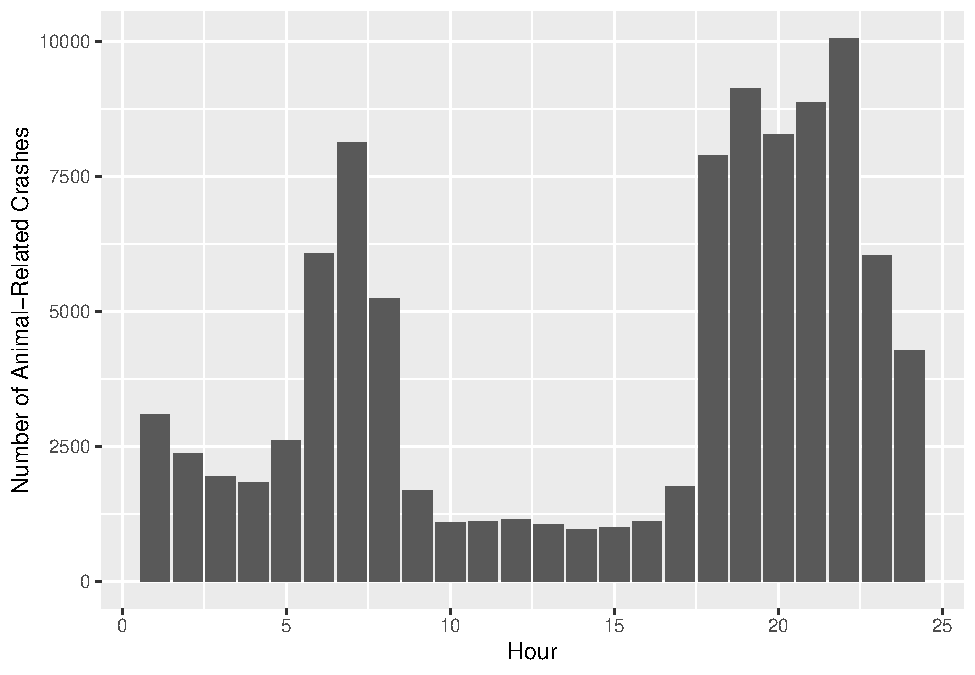
\includegraphics[width=0.9\columnwidth]{CAUSE_files/figure-latex/unnamed-chunk-1-1} \end{center}

After cleaning the data, our analysis focused on how time of the day when car crashes happen. We hypothesize that more crashes will happen in the morning and evening as the driver is travelling into the sun and has to deal with sun glare, preventing them from seeing clearly.

\hypertarget{data-extraction}{%
\subsection{Data Extraction}\label{data-extraction}}

Because evening and morning times are variable throughout the year, one must look at when the sun is rising and setting. Because this data was not included in the original data set, the data was scraped from Time and AS (1995-\/-). The data includes sunrise and sunset times for Ames, Iowa in 2020. The reasoning behind using Ames was that it is the nearest major town to the geographical center of Iowa. This would limit variation of sunrise and sunset times based on location. For approximately every 70 miles, there is a one minute change in sunrise and sunset times. By using Ames, these discrepancies to under three minutes. The year 2020 was chosen because it is the most recent leap year and would provide meaningful data for February 29.

Figure \ref{fig:timeanddate} shows an example table from timeanddate that was used for the data collection is as follows:

\begin{figure}

{\centering 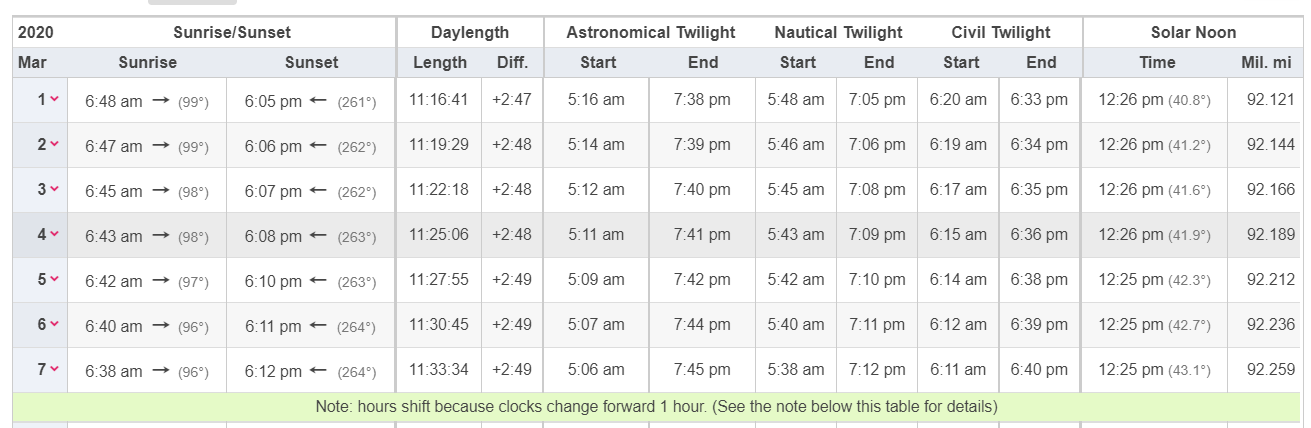
\includegraphics[width=0.9\columnwidth]{../images/paste-5719206D} 

}

\caption{Example table of the data collected for sunrise and sunset times.}\label{fig:timeanddate}
\end{figure}

Using a function, the data was extracted for each month in 2020 and joined with the original crash data set.

\hypertarget{sunrisesunset-analysis-1}{%
\subsection{Sunrise/Sunset Analysis}\label{sunrisesunset-analysis-1}}

Figure \ref{fig:sunrise} shows the minutes from sunrise compared to number of crashes, with a line denoting when the sunrise time is:

\begin{figure}

{\centering 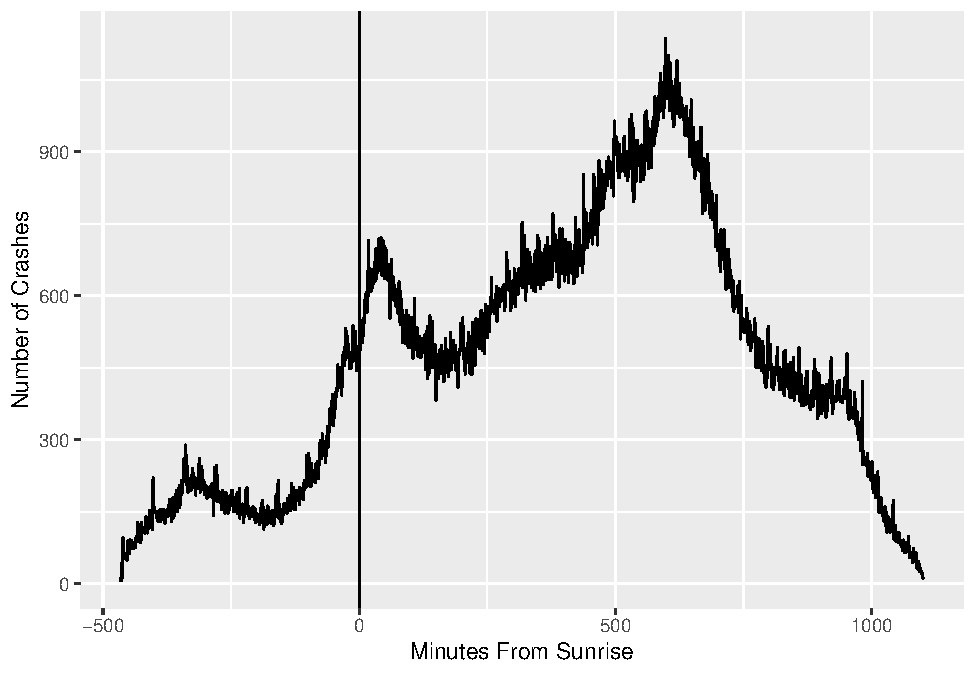
\includegraphics[width=0.9\columnwidth]{CAUSE_files/figure-latex/sunrise-1} 

}

\caption{A graph of all crashes by the difference between crash time and sunrise.}\label{fig:sunrise}
\end{figure}

This clearly appears that there is a small spike, starting right before the sun rises.

There also seems to be a noticeable spike around 750 minutes after sunrise time. This likely corresponds to sunset time, so it is only logical to look at how sunset time affects car crashes. Figure \ref{fig:sunset} shows the minutes away from sunset, with a line denoting where the sun sets.

\begin{figure}

{\centering 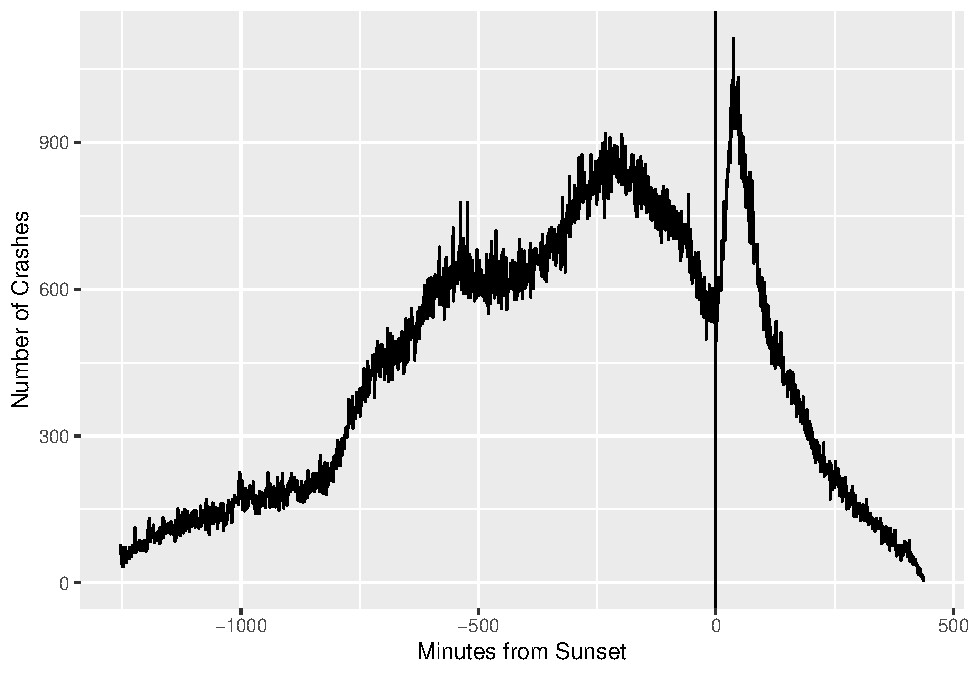
\includegraphics[width=0.9\columnwidth]{CAUSE_files/figure-latex/sunset-1} 

}

\caption{A graph of all crashes by the difference between crash time and sunset}\label{fig:sunset}
\end{figure}

There appears to be a pretty drastic jump right after the sun sets. According to the Council (2020), driving at dusk is extremely dangerous, as one's eyes take time to adjust to the relative darkness, shadows hide animals and road features, and driver sometimes fail to turn on their headlights. This may be a reason why there is such a strong correlation between sunset time and a spike in car crashes.

\hypertarget{daylight-analysis}{%
\subsection{Daylight Analysis}\label{daylight-analysis}}

One point of note is looking into how the length of the day affects car crashes. The following graph shows the number of crashes based on the length of the day. A line of best fit was added to the graph using LOESS smoothing.

There seems to be more variability in earlier months, but overall a downward trend.

\begin{figure}

{\centering 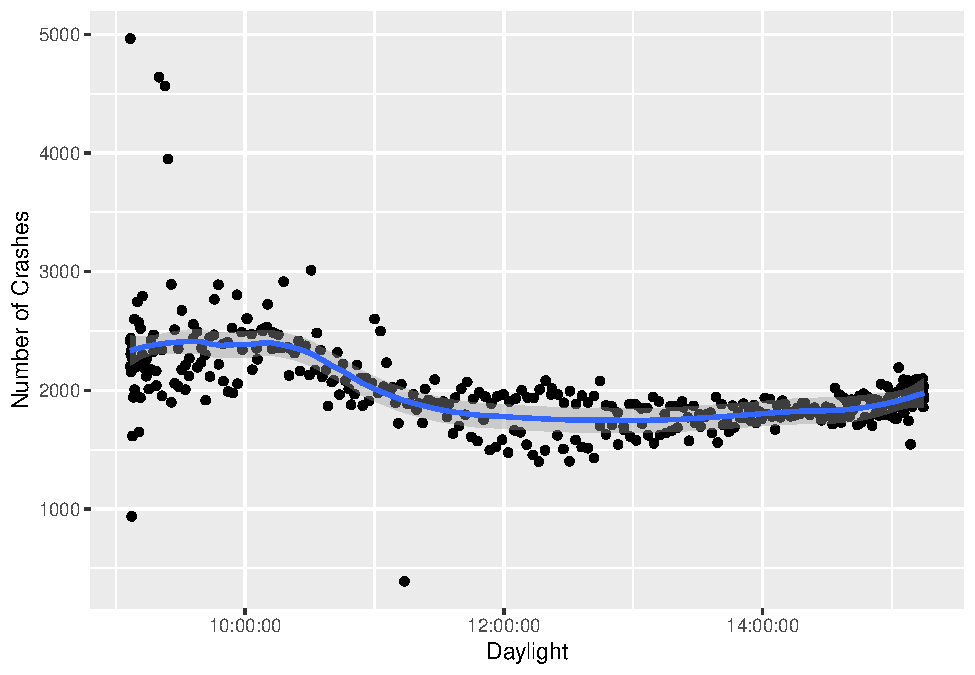
\includegraphics[width=0.9\columnwidth]{CAUSE_files/figure-latex/unnamed-chunk-5-1} 

}

\caption{A graph of all crashes based on the length of the day with a line fitted using LOESS smoothing}\label{fig:unnamed-chunk-5}
\end{figure}

There is very clearly a downward trend, showing that there is a correlation to fewer daylight hours and more crashes.

\hypertarget{conclusion}{%
\subsubsection{Conclusion:}\label{conclusion}}

A number of conclusions can be drawn from this data analysis. First, we can conclude that there is a correlation between sunset and sunrise time and frequency of crashes. The 30-minute window after the sun sets, especially, is correlated with an increase in crashes in Iowa. There is also a correlation between higher numbers of crashes and fewer daylight hours, but this may be correlated with the winter months being more dangerous for drivers. For future research, we would like to to further look into how rush hour traffic may affect these trends.

\hypertarget{alcohol-analysis}{%
\section{Alcohol Analysis}\label{alcohol-analysis}}

For my analysis, I would like to look into the relationship between alcohol and car crashes. I especially want to look into how the severity of car crashes and alcohol are related and what times are the most dangerous in terms of drunk drivers.

The main data set has a variable titled ``Drug or Alcohol'' with eight different levels. However, only two of these levels signify that substances were not involved. Because of this I created a helper variable titled ``Drug\_Usage'' that is TRUE when there are substances involved and FALSE when there is none present.

In order to perform further calculations, I also created some helper variables containing the total of crashes with and without alcohol, respectively.

After that, I found the average property damage that results from crashes with and without drunk driving. As I expected, drunk crashes do cause more damage, almost \$3000 more on average.

\begin{center}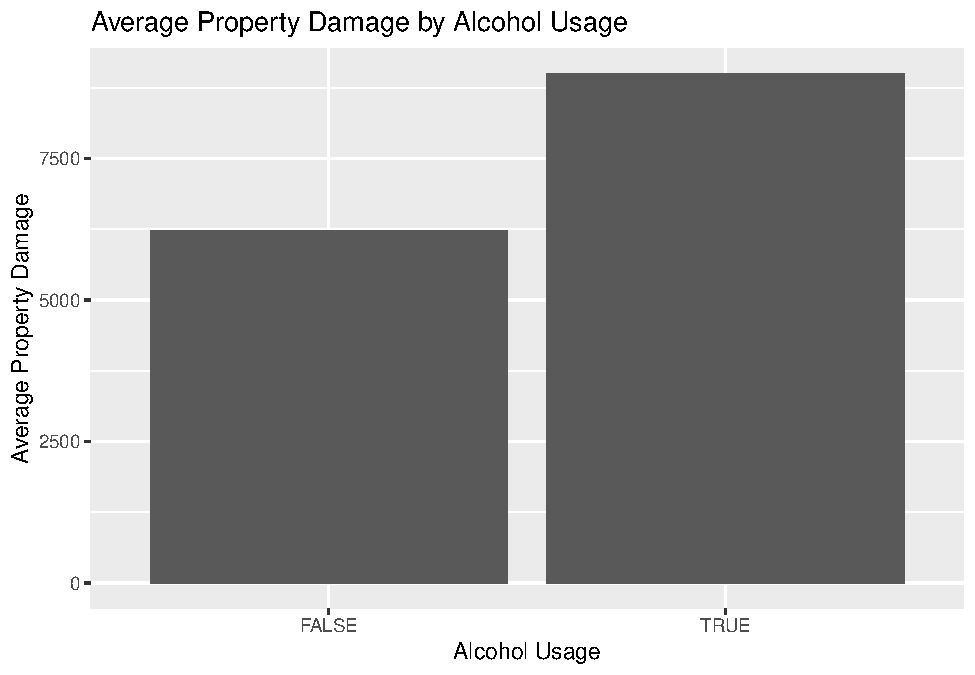
\includegraphics[width=0.9\columnwidth]{CAUSE_files/figure-latex/unnamed-chunk-9-1} \end{center}

I also looked at the average fatalities per crash with and without alcohol. The actual values of the averages aren't super intuitive, as they are small decimals, but finding the average rate of fatalities is much more useful. When doing so, fatalities occur in sober crashes about 1 in 217 crashes, while fatalities in drunk crashes occur at about 1 in 20. This difference in fatality is expected, but I am shocked at how much higher it truly is.

Next, I decided to look into how time of day affects drunk driving. I plotted sober and drunk crashes and tried to find a pattern.

\begin{center}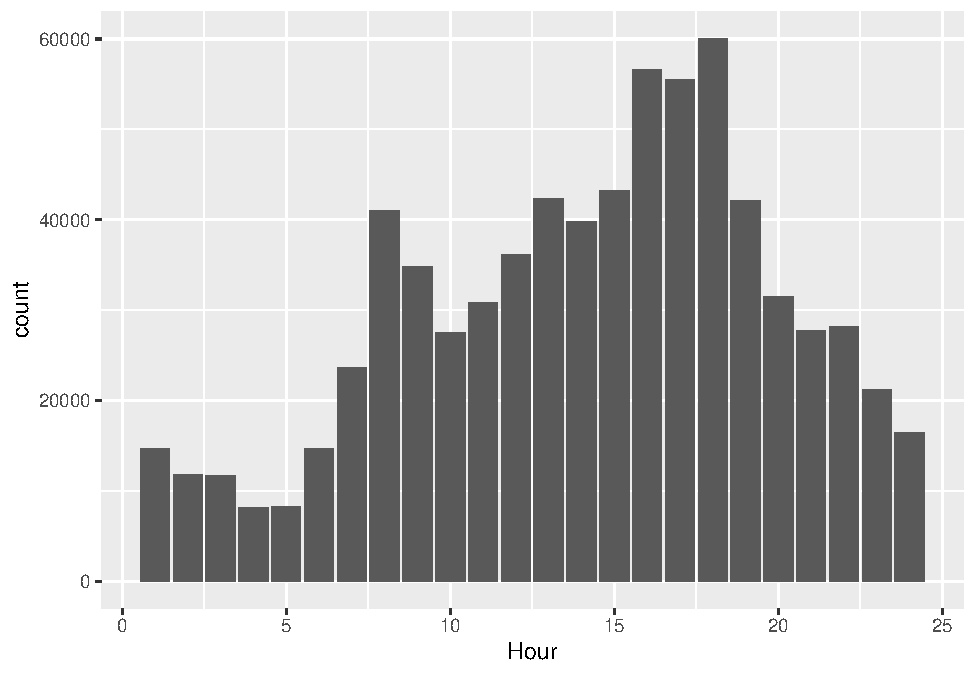
\includegraphics[width=0.9\columnwidth]{CAUSE_files/figure-latex/unnamed-chunk-11-1} \end{center}

\begin{center}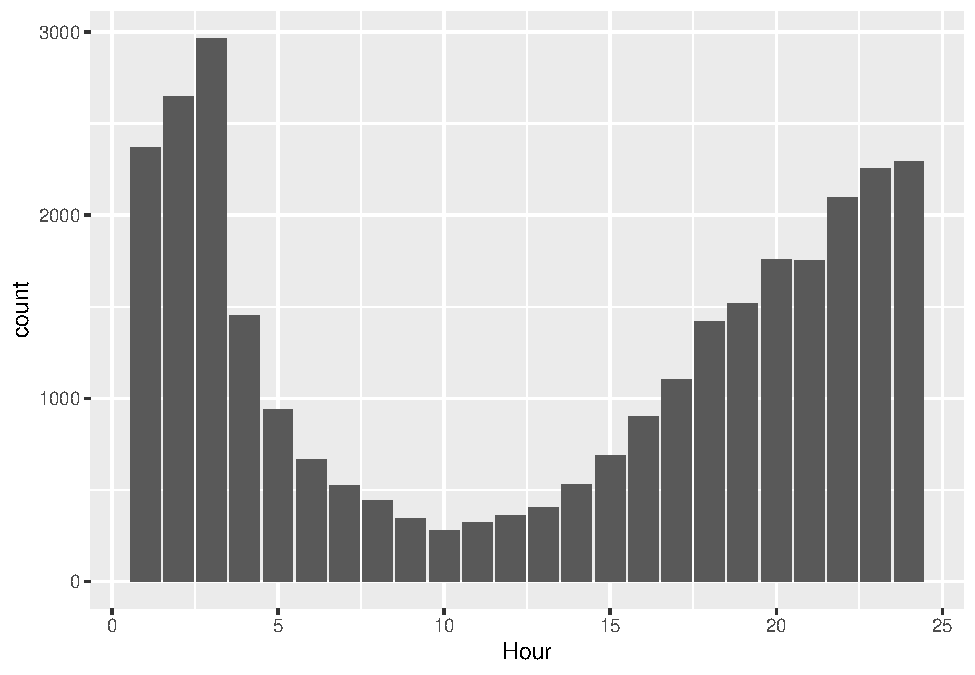
\includegraphics[width=0.9\columnwidth]{CAUSE_files/figure-latex/unnamed-chunk-11-2} \end{center}

After that, I decided to try and find what percentage of crashes that occur during late night hours involve alcohol. To do so, I created a helper variable containing all crashes that occurred between 10 P.M. and 4 A.M.

The next unit of time I decided to look at was day of the week. I expected to see a large spike on weekends, especially on Friday and Saturday. To do so, I once again plotted both sober and drunk crashes by day of the week and compared them.

\begin{center}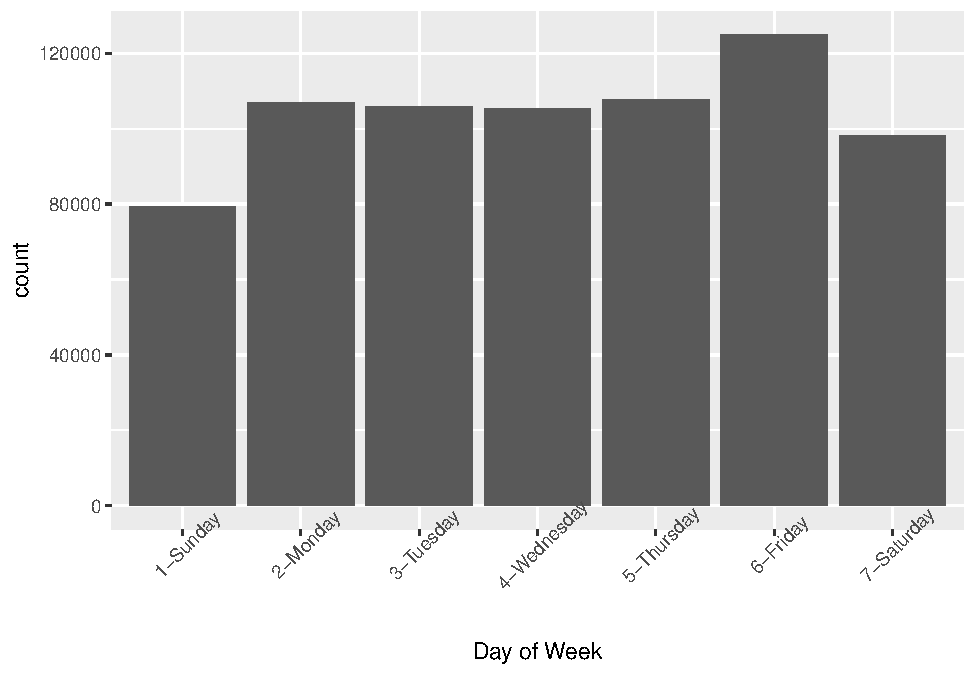
\includegraphics[width=0.9\columnwidth]{CAUSE_files/figure-latex/unnamed-chunk-14-1} \end{center}

\begin{center}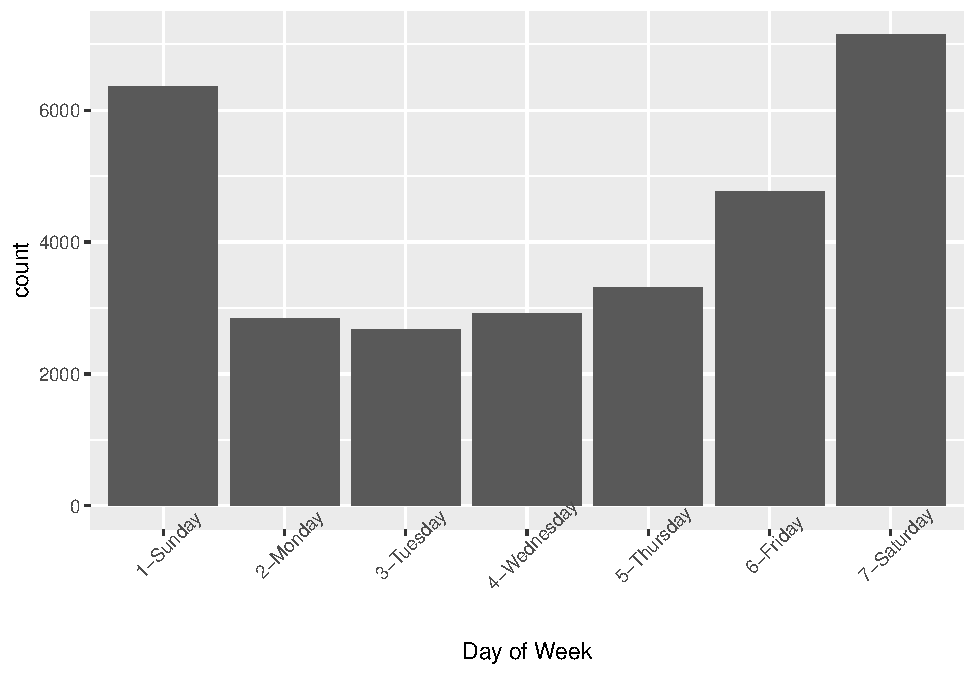
\includegraphics[width=0.9\columnwidth]{CAUSE_files/figure-latex/unnamed-chunk-14-2} \end{center}

Finally, I looked at crashes by day of the year. There is no real pattern in by day of the year, but there are a few outliers. Both New Year's day and the Fourth of July have a very large amount of drunk crashes in comparison to the rest of the year. This first graph shows all drug-related crashes:

\begin{center}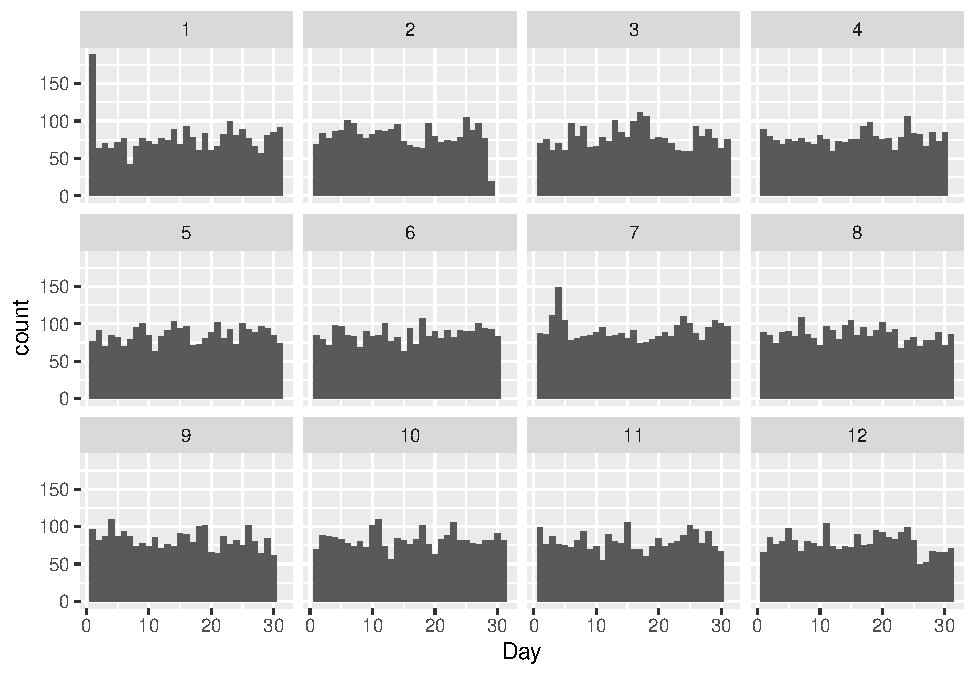
\includegraphics[width=0.9\columnwidth]{CAUSE_files/figure-latex/unnamed-chunk-15-1} \end{center}

Figure \ref{fig:avgcrashes} shows the average number of crashes in Iowa by day of year.

\begin{figure}

{\centering 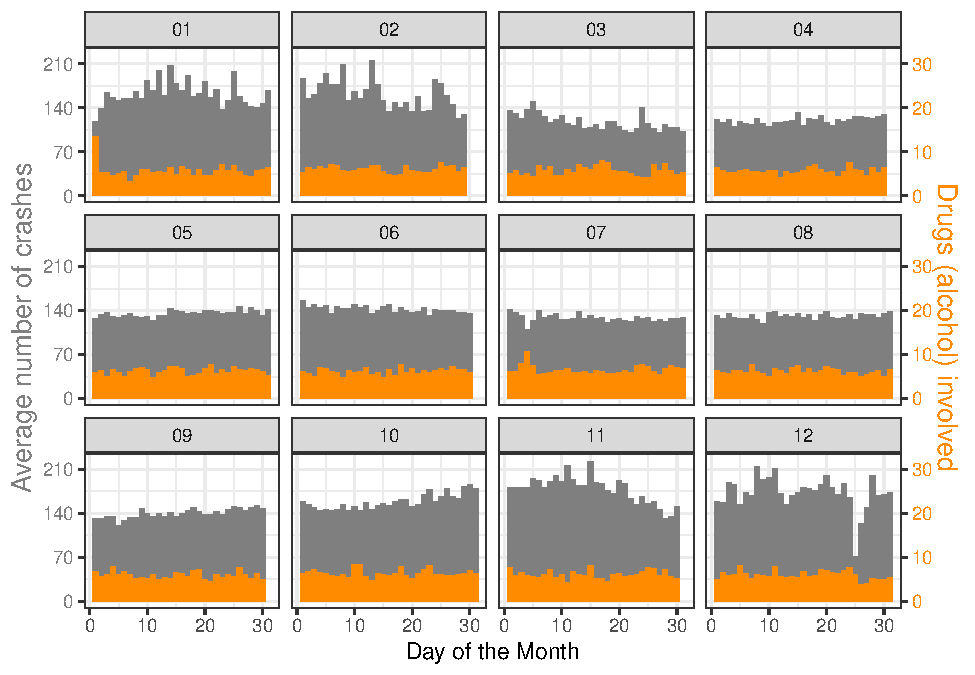
\includegraphics[width=\columnwidth]{CAUSE_files/figure-latex/avgcrashes-1} 

}

\caption{Average number of crashes by day of the year. Spring and summer months see on average fewer crashes than the rest of the year. From November to February, we see an increased variability in the number of crashes -- this is likely due to bad weather days in some of the years. There is a clear holiday effect in the number of crashes: Jan 1, July 4, Thanksgiving, and, in particular, Christmas day and the day after have a much-reduced number of crashes. However, both New Year's day and the Fourth of July have a very large amount of drunk crashes in comparison to the rest of the year (shown in orange). }\label{fig:avgcrashes}
\end{figure}

The fact that New Year's day has triple the amount of drug-involved crashes as any other day is particularly scary because January first has the lowest amount of overall crashes in the month of January.

\begin{center}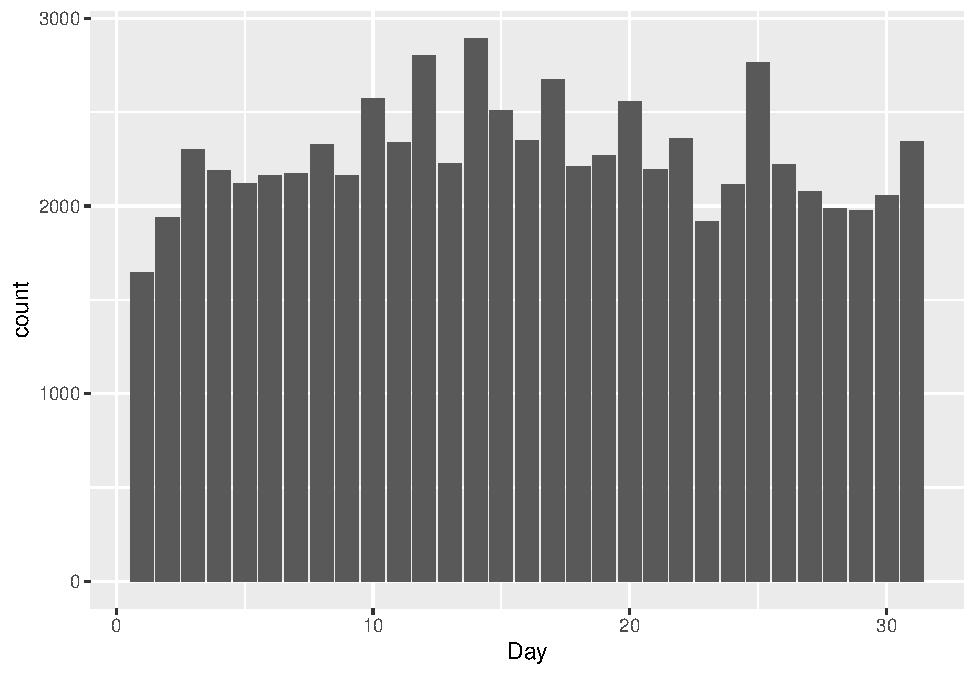
\includegraphics[width=0.9\columnwidth]{CAUSE_files/figure-latex/unnamed-chunk-16-1} \end{center}

\hypertarget{conclusion-1}{%
\subsection{Conclusion}\label{conclusion-1}}

\begin{enumerate}
\def\labelenumi{\arabic{enumi}.}
\item
  Alcohol drastically increases the danger and severity of crashes: fatalities, injuries, and property damage all occur at an increased rate.
\item
  Nighttime and Friday and Saturday nights are the times with the most drunk driving, so it may be wise to avoid the roads at those times.
\item
  The worst nights to drive on are New Year's Eve and the Fourth of July, as they by far have the most drunk accidents of any other days in the year.
\end{enumerate}

\hypertarget{conclusion-2}{%
\section{Conclusion}\label{conclusion-2}}

The conclusion goes here.

\clearpage

\hypertarget{appendix}{%
\section*{Appendix}\label{appendix}}
\addcontentsline{toc}{section}{Appendix}

\textbf{HH: move the next paragraph to the appendix}

Data cleaning included changing empty strings and illogical values into NA values. Day, month, and year values were extracted using R's lubridate package. Latitude and longitude was columns were also created from the `Position' column to further explore where crashes happen in Iowa.

\hypertarget{data-cleaning}{%
\section{Data Cleaning}\label{data-cleaning}}

\hypertarget{data-on-sunsets-and-sunrises}{%
\section{Data on Sunsets and Sunrises}\label{data-on-sunsets-and-sunrises}}

\clearpage

\hypertarget{references}{%
\section*{References}\label{references}}
\addcontentsline{toc}{section}{References}

\hypertarget{refs}{}
\begin{CSLReferences}{1}{0}
\leavevmode\vadjust pre{\hypertarget{ref-duskdawn}{}}%
Council, Delaware Safety. 2020. {``Safe Driving Dusk and Dawn.''} \url{https://delawaresafety.org/resources/Documents/Safety\%20Documents/Safe\%20Driving\%20-\%20\%20Dusk\%20and\%20Dawn.pdf}.

\leavevmode\vadjust pre{\hypertarget{ref-iowadot}{}}%
Iowa Department of Transportation. 2022. {``Iowa Motor Vehicle Crashes - 1925 to 2020.''} \url{https://iowadot.gov/mvd/stats/crashhistory.pdf}.

\leavevmode\vadjust pre{\hypertarget{ref-timeanddate}{}}%
Time, and Date AS. 1995-\/-. {``Ames, Iowa, USA - Sunrise, Sunset, and Daylength in 2020.''} \url{https://www.timeanddate.com/sun/usa/ames}.

\end{CSLReferences}

\end{document}

